\section{Tainting dependencies}
\label{sect:impl:tainting_deps}
``Tainting dependencies'' is a method of translating XQuery queries to
relational algebra. The semantics of this method is described in detail
throughout section \ref{sect:trans:taintingDependencies}. This section
describes an implementation of a subset of this method which is capable of
translating simple FLWOR expressions, sequences, and variables. 

\subsection{FLWOR expressions}
The translation process for FLWOR expressions were outlined in section
\ref{sect:trans:TD:simpleFLWOR}. Consider inference rule
\ref{rule:trans:TD:forbind} on page \pageref{rule:trans:TD:forbind}. This
inference rule states how to translate and bind an iterator variable in a
for-clause in a FLWOR expressions. The implementation of this inference rule is
shown in figure \ref{fig:impl:td:varbindfor}. This excerpt includes two visitor
methods. First a for-clause is visited, and the child is flagged as a FLWOR
tuplet definition (lines 1 through 7). Next a dollar sign is visited (which
carries the meaning of a variable in the abstract syntax tree). If the child
count is more than one, it is an assignment. Note that the
\texttt{isIterationVar} flag is \textit{true} if this assignment is a tuple
definition as flagged earlier.

Then, if this is an assignment and a tupled definition, the right-hand side of
the assignment is translated, and the symbol is entered into a symbol table.
Note that the creation of the project operator is required by inference rule
\ref{rule:trans:TD:forbind}.

This example can be better understood if seen in context of an abstract syntax
tree example. Considering the example in figure \ref{fig:impl:td:flwor2}. Here
the \textit{AST\_FORCLAUSE} node will be visited by the
\texttt{visitAST\_FORCLAUSE()} method in the visitor and the
\texttt{isFlworTupleDef} flag will be set to \textit{true}. Then the variable
node (the dollar sign) will be visited by the \textit{visitDOLLARSi()} method,
and the translation of the for clause is completed.

\begin{figure}[!htp]
\begin{center}
\lstset{language=Java,numbers=left}
\begin{lstlisting}
    public TraverseReturn visitAST_FORCLAUSE(XQFTTree tree) {
        
        ((XQFTTree)tree.getChild(0)).setFlworTupleDef(true);
        acceptThis(tree.getChild(0));

        return null;
    }
    .
    .
    .
    
    public TraverseReturn visitDOLLARSi(XQFTTree tree) {
        
        boolean isIterationVar = tree.isFlworTupleDef();
        
        String varName = tree.getChild(0).getText();
        
        // Assignment?
        if (tree.getChildCount() > 1) {
            
            // Visit children on the right side of the assignment
            TraverseReturn tr = acceptThis(tree.getChild(1));
            
            // Required for tainting deps method
            Project project = new Project(
                "[" + varName + "numb, value]", 
                tr.getOperatorTree());

            // Assign metadata
            tr.setOperatorTree(project);
            tr.setSingleton(true);
            
            // Enter into symbol table
            SymTabEntry tmp = Scope.set(tree.getChild(0).getText(), 
                                  tr, isIterationVar);
            
            if (isIterationVar) {
               Scope.getInstance().setCurrentIterVar(
                                       new VarRef(tmp.getName()));
            }
            
            return tr;
        }
        .
        .
        .
\end{lstlisting}
  \caption{Translation and binding of iteration variables}
  \label{fig:impl:td:varbindfor}
\end{center}
\end{figure}

%\usepackage{graphics} is needed for \includegraphics
\begin{figure}[!htp]
\begin{center}
  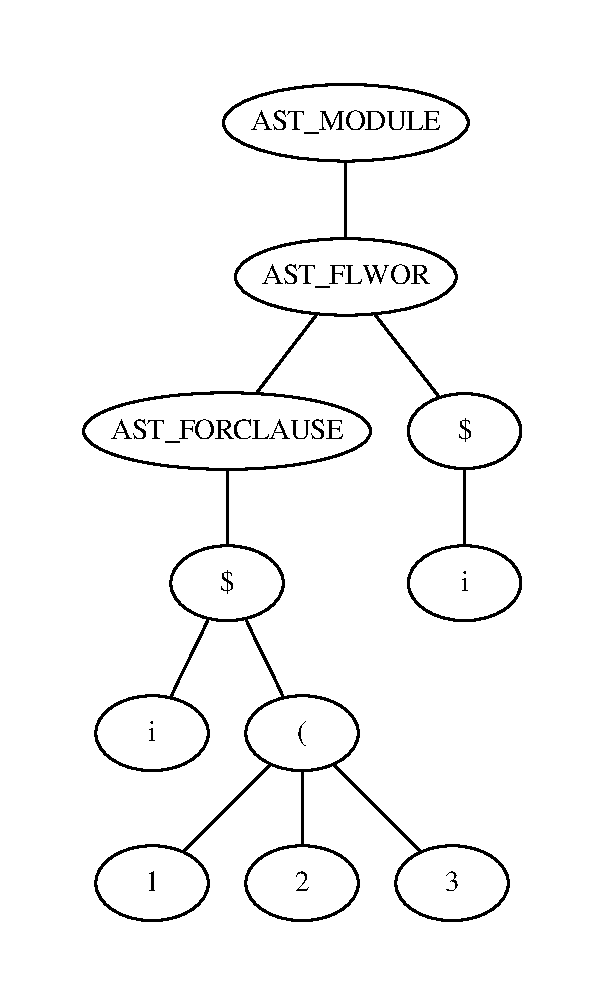
\includegraphics[scale=0.4]{img/graphs/flwor2}
  \caption{FLWOR syntax tree example}
  \label{fig:impl:td:flwor2}
\end{center}
\end{figure}

Following the translation of the for-clause, the return clause is translated in
a similar manner. However this translation is slightly more complicated. The
translation is dependent on whether the return clause contains code which
references the current iteration variable. If this is the case, then a
translation which applies tainting given by the rule in figure
\ref{eq:trans:TD:taint} page \pageref{eq:trans:TD:taint} must be used. In
particular, the rule in figure \ref{rule:trans:TD:returnTaint} shown on page
\pageref{rule:trans:TD:returnTaint} must be applied (which implies the former).

\begin{figure}[!htp]
\begin{center}
\lstset{language=Java,numbers=left}
\begin{lstlisting}
// Sort and partition fields
String[] sortBy = {Scope.getInstance().getCurrentIterVar().getName() 
		          + "numb", "index"};
String[] partitionBy 
	= new String[returnClauseResult.getVarRefs().size() - 1];

// Calculate variable references
VarRefSet prevVarRefs 
	= (VarRefSet)returnClauseResult.getVarRefs().clone();         
prevVarRefs.remove(Scope.getInstance().getCurrentIterVar());

int i = 0;
for (VarRef ref : prevVarRefs) {
    partitionBy[i] = ref.getName();
    i++;
}

// Construct MQL
Numberate numberate = new Numberate("index", 
                                    sortBy, 
                                    partitionBy, 
                                    returnClauseResult.getOperatorTree());

// Construct result
TraverseReturn result = new TraverseReturn();
result.setSingleton(false);
result.setVarRefs(returnClauseResult.getVarRefs());
result.setOperatorTree(numberate);

// Remove current iter var from varrefs
result.getVarRefs().remove(Scope.getInstance().getCurrentIterVar());

Scope.pop();
return result;
\end{lstlisting}
  \caption{Translation of a return clause with a reference to the current
  iteration variable}
  \label{fig:impl:td:for_return_withref}
\end{center}
\end{figure}

Figure \ref{fig:impl:td:for_return_withref} shows how this has been
implemented. Note that the code in this example is executed if and only if
there is a reference to the iteration variable in the return clause.

If there is no reference to the current iteration variable, then the
translation is done as usual per rule 

\subsection{Sequences}
\label{sect:impl:td:seq}
The translation process for sequence construction is described in section
\ref{sect:trans:TD:seqBuild}. This rule is somewhat complex, and requires
collecting all variable references from all children before performing the
actual translation. Furthermore, for any variable reference in a left-most
child, this variable reference must taint all right-most children. This process
is shown in figure \ref{fig:impl:td:seq_constr_tainting_siblings}.

\begin{figure}[!htp]
\begin{center}
\lstset{language=Java,numbers=left}
\begin{lstlisting}
for (TraverseReturn childResult : childResults) {
    VarRefSet varRefsDiff;
    Operator expr = childResult.getOperatorTree();
    
    VarRefSet tmp = childResult.getVarRefs();
    varRefsDiff = (VarRefSet)varRefs.clone();
    varRefsDiff.removeAll(tmp);

    for (VarRef varRef : varRefsDiff) {
        Project project = new Project(varRef.getName() + "numb", 
                Scope.get(varRef.getName()).getTraverseReturn().getOperatorTree());
        
        Cross cross = new Cross(project, expr);
        expr = cross;
    }

    if (childResult.isSingleton()) {
        expr = new Project("sprIdx="+(c+1)+",index,value", expr);
    }
    else {
        expr = new Project("sprIdx="+(c+1)+",value", expr);
    }
    operators.add(expr);
    c++;
}
\end{lstlisting}
  \caption{Tainting siblings in a sequence construction}
  \label{fig:impl:td:seq_constr_tainting_siblings}
\end{center}
\end{figure}

This will propagate tainting throughout the siblings as required. When this
procedure is complete, the operator tree in the \texttt{operators} variable is
wrapped in a \textsf{union()} operator. Etc.

\begin{itemize}
  \item behandler parantes istf. komma for sekvenser (ref spec) 
\end{itemize}

\subsection{If-then-else}
TODO: Skrive om if-then-else? comparisons??

